\subsection{Facade}
Viene usato per fornire un’interfaccia unica e semplice per un sotto sistema complesso.
In questo modo vengono semplificate le varie dipendenze tra i sotto sistemi, senza nascondere le funzionalità di basso livello.
Di conseguenza:
\begin{itemize}
\item Diminuiscono le classi del sotto sistema con il quale il client deve interagire;
\item C’è un accoppiamento lasco tra i sotto sistemi, senza dipendeze circolari;
\item Viene introdotto un single point of failure;
\item \`{E} necessario prestare attenzione al dimensionamento della classe Facace che non deve essere troppo grande.
\end{itemize}
\begin{figure}[ht]
    \centering
    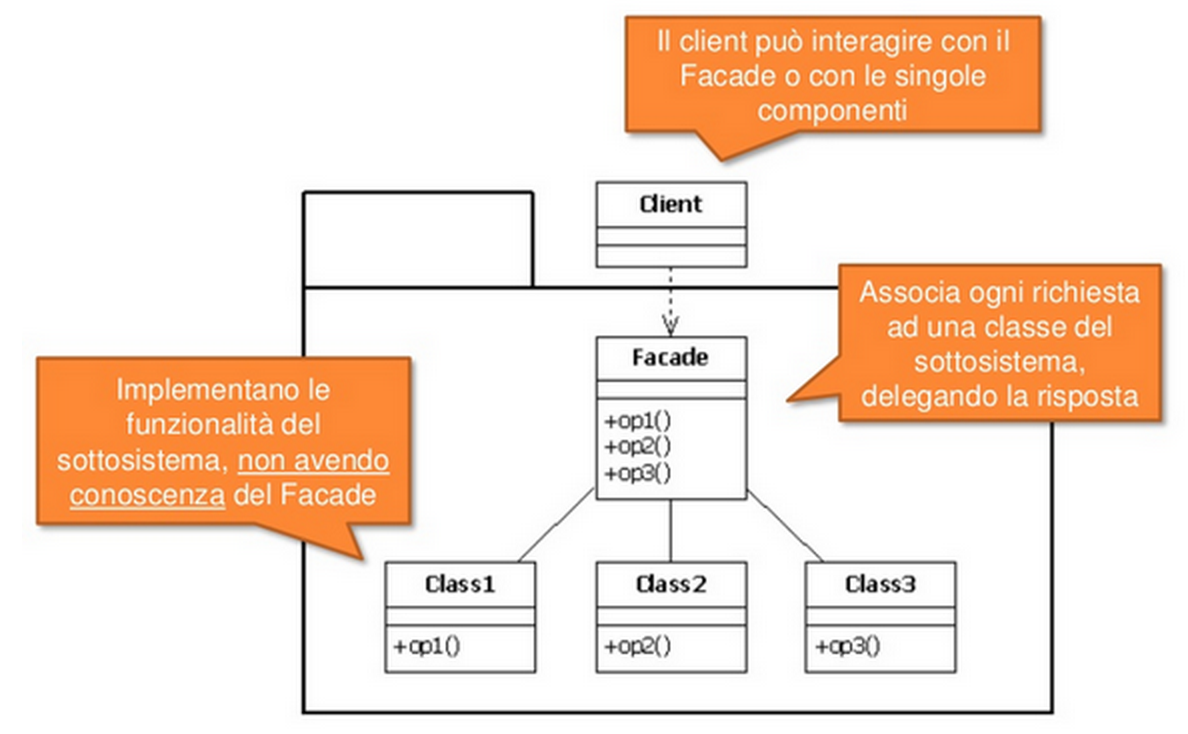
\includegraphics[width=0.8\textwidth]{immagini/facade.png}
    \caption{Facade}
\end{figure}
\FloatBarrier